% {Youssouph Cissokho}
\section{Applications}\label{Section:6}
We end this report with  an experimental comparison of some of the outlier detection methods discussed in the preceding sections. 
\newl \textbf{Data pre-preprocessing:} all datasets have been normalized, and qualitative variables have been removed.
\newl \textbf{Algorithms:} we test $4$ algorithms, namely  \textbf{Local Outlier Factor}  (LOF), \textbf{Isolation Forest} (iF), \textbf{$k$ Nearest Neighbours} ($k$NN) and \textbf{Principal Component Analysis} (PCA). The default parameters are used in all cases.  \newl
\textbf{Datasets:}
\noindent \textbf{a) Dataset 1: Airlines:} includes information on all domestic flights in the USA in 2019, such as departure time, arrival time, origin airport, destination airport, etc. available  \href{https://www.transtats.bts.gov/DL_SelectFields.asp?Table_ID=}{\textcolor{blue}{\underline{here}}}. The purpose is to analyse delays in departures and/or arrivals of flights. Indeed, a flight is considered to be "on time" \textbf{if it arrives less than 15 minutes later than the indicated time} in the carrier's computer reservation systems (CRS). Therefore, \textbf{anomalies are flights with chronic delays}. To do this, a sample of $500$ flights departing from Chicago O'Hare Airport (ORD) is extracted and average delay times are calculated in relation to airport arrival times. The average arrival time is calculated for all flights landing at a given airport.\textbf{ The anomalies are therefore the airports that show unusual average delays.}
\begin{figure}
    \centering
    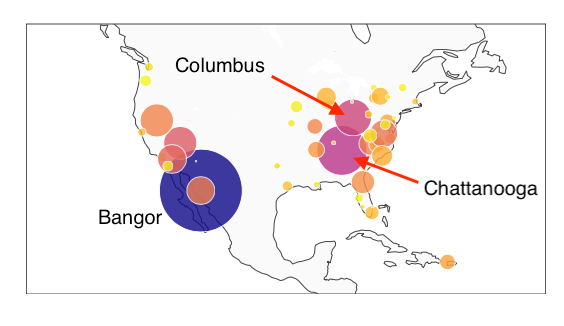
\includegraphics[width=.50\textwidth]{\MainFolder/Images/vols1.png}
    %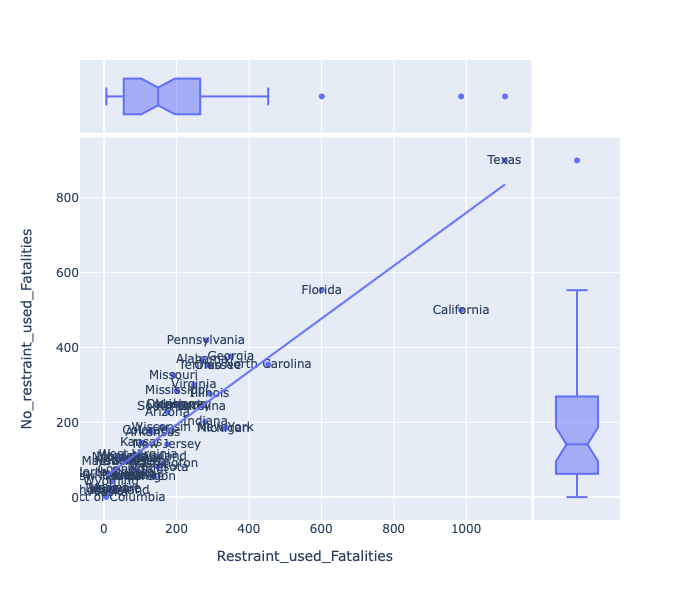
\includegraphics[width=.40\textwidth]{\MainFolder/Images/Fatal1.png}
    \caption{Scatterplot of arrival delays on the map with the variable ARR\_DELAY as the size of the balls.}%\hrule
    \label{fig20}.
\end{figure}
\noindent Figure \ref{fig20}, shows airports \textbf{Bangor, Chattanooga, Columbus, etc.} which show unusual average delays (very high) and therefore are likely to be abnormal. Some methods have therefore been analysed in detail, the results are in figure \ref{fig21}.\newl
\begin{figure*}[ht]
    \centering
     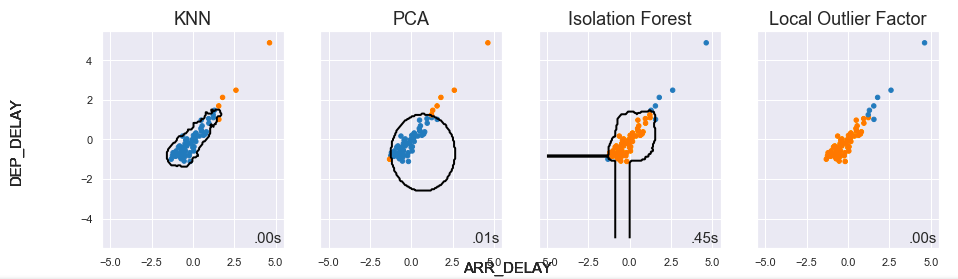
\includegraphics[width=1\textwidth]{\MainFolder/Images/Voll.png}\label{fig02}.
    \caption{Airports detected as outliers by PCA, KNN, Isolation Forest and LOF.}%\hrule
    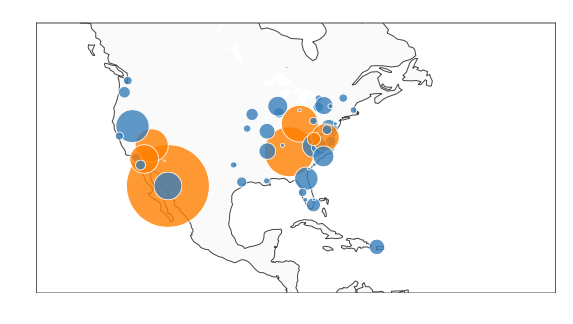
\includegraphics[width=.45\textwidth]{\MainFolder/Images/vol1PCA.png}
    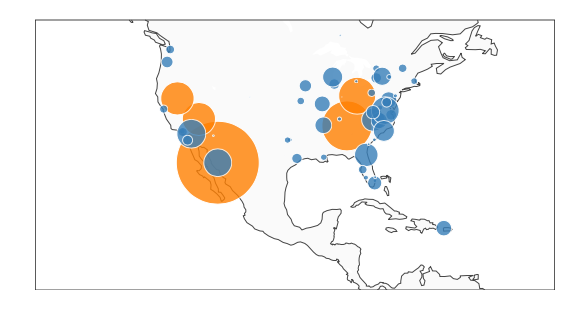
\includegraphics[width=.450\textwidth]{\MainFolder/Images/vols1KNN.png}\\
    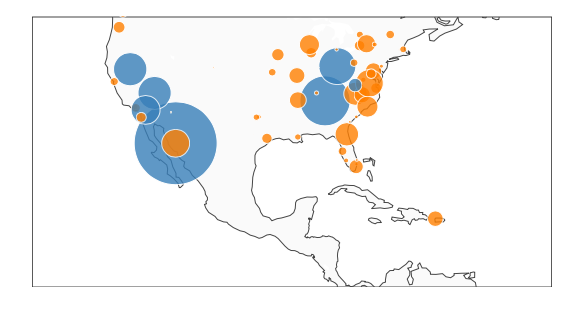
\includegraphics[width=.45\textwidth]{\MainFolder/Images/volsIsoFor.png}
    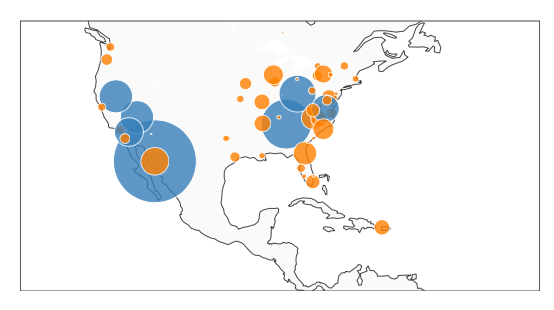
\includegraphics[width=.450\textwidth]{\MainFolder/Images/volsLOFpng.png}
    \caption{Airports detected as outliers by PCA (top left), KNN (top right), Isolation Forest (bottom left) and LOF (bottom right)}%\hrule
    \label{fig21}
\end{figure*}
\noindent\textbf{Analysis of the results:} 
In Figures \ref{fig21}, you can see outliers as detected by the different techniques. The blue circles represent airports without abnormal behavior, while the orange circles represent airports with abnormal behavior for (\textbf{PCA and KNN}) and inversely for (\textbf{IsolationForest and LOF}). \textbf{Average arrival time defines the size of the circles}. Some airports are identified as outliers by all methods: the airport of \textbf{Bangor, Columbus and Las vegas} while \textbf{Chattanooga} is only detected by KNN, see Table \ref{fig2w}. However, \textbf{Bangor} is the airport with the longest arrival delay (141 minutes). This delay can be explained by a long process and poor infrastructure conditions at the airport or delays caused by bad weather or other reasons. What is certain is that it deserves further investigation.

\afterpage{\FloatBarrier}

\noindent \textbf{b) Dataset 2: Fatal Accidents:}
 is a data representing fatal accidents involving only occupants of passenger cars and light trucks in  United States. \textbf{These accidents involve any activity that may divert a person's attention from the main task of driving, such as texting, using a cell phone, eating and drinking, grooming, using a navigation system, tuning the radio, etc.} available  \href{https://www.bts.dot.gov/content/passenger-car-and-light-truck-occupants-killed-and-restraint-use}{\textcolor{blue}{\underline{here}}}. \newl
\noindent \textbf{Analysis of the results:}
A visual analysis of Figure \ref{fig2}, shows that there are countries that stand out from the rest with a high number of fatalities in those countries. On the other hand, the boxplot  also tells us that these countries are abnormal (outliers), these countries are \textbf{Texas, california, Florida}. Further analysis is conducted to corroborate the previous results. These methods are \textbf{ KNN, PCA, LOF and Isolation Forest}. The result is presented in Figure \ref{fig2b}. 
\begin{figure}
    \centering
    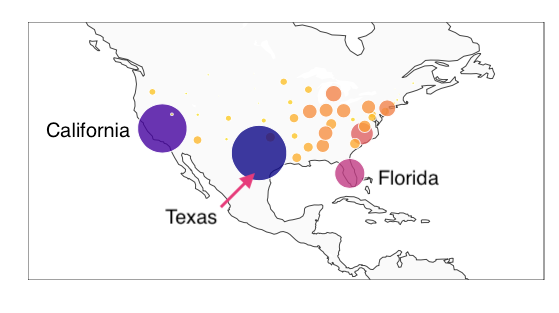
\includegraphics[width=.5\textwidth]{\MainFolder/Images/fat1png.png}
    %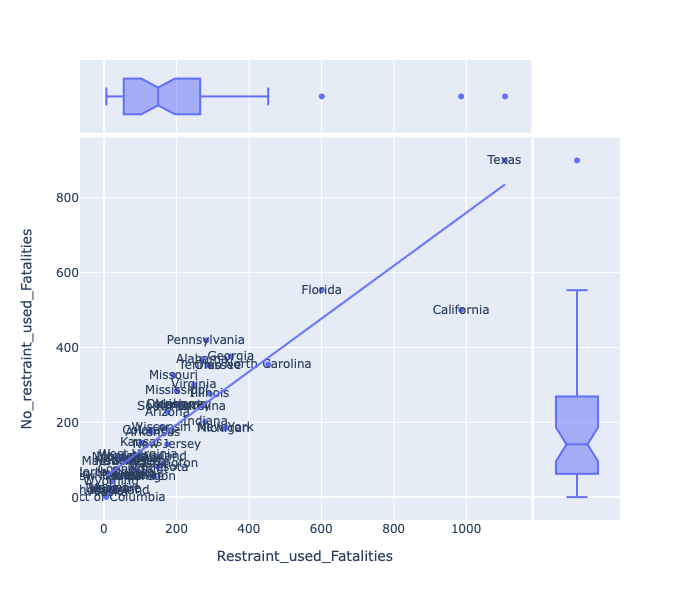
\includegraphics[width=.40\textwidth]{\MainFolder/Images/Fatal1.png}
    \caption{Point cloud of fatal accidents on the map with the variable Restraint\_used\_Fatalities as the size of the balls.}%\hrule
    \label{fig2}
\end{figure}
%
%
\begin{table}
\centering
 \begin{tabular}{||c c c c c||} 
 \hline
 &  KNN & PCA & IsolForest & LOF\\ [0.5ex] 
 \hline\hline
Bangor & $\checkmark$ & $\checkmark$  & $\checkmark$ & $\checkmark$ \\ 
 Las vegas & $\checkmark$ & $\checkmark$  & $\checkmark$ & $\checkmark$ \\
Columbus & $\checkmark$ & $\checkmark$  & $\checkmark$ & $\checkmark$ \\
 Chattanooga & $\checkmark$ & $\times$  & $\times$ & $\times$ \\ [1ex] 
 \hline
 \end{tabular}
 \caption{Summary of results.}
 \label{fig2w}
\end{table}
\begin{table}
\centering
 \begin{tabular}{||c c c c c||} 
 \hline
 &  KNN & PCA & IsolForest & LOF\\ [0.5ex] 
 \hline\hline
Texas & $\checkmark$ & $\checkmark$  & $\checkmark$ & $\checkmark$ \\ 
 California & $\checkmark$ & $\checkmark$  & $\checkmark$ & $\checkmark$ \\
Florida & $\checkmark$ & $\checkmark$  & $\checkmark$ & $\checkmark$ \\
 North Carolina & $\checkmark$ & $\times$  & $\times$ & $\times$ \\ [1ex] 
 \hline
 \end{tabular}
 \caption{Summary of results.}
\end{table}

\noindent\textbf{c) Dataset 3: Temperatures in Australia:}.
This dataset describes the daily minimum temperatures over 10 years (1981-1990) in the city of Melbourne, Australia, see Figure \ref{fig2t}. Units are in degrees Celsius and there are $3650$ observations. The source of the data is attributed to the Australian Bureau of Meteorology and can be downloaded at \href{https://machinelearningmastery.com/time-series-data-visualization-with-python/}{\textcolor{blue}{\underline{here}}}. A large number of applications generate temporal data sets. For example, in our daily lives, various types of records such as credit, personnel, finance, justice, medicine, etc., are all temporal. This underscores the need for an organized and detailed study of outliers in relation to this temporal data \cite{A5}. Anomalies in the data series cause unexpected spikes, declines, changes in trend, or changes in level. For a univariate series, the problem can be considered supervised or unsupervised. In the first, two limits are calculated (upper and lower bounds), all observations beyond these limits are considered abnormal. In the following example, the unsupervised method is considered.\newl
\noindent\textbf{Analysis of the results} 
Figure \eqref{fig2t1} shows the results of four methods \textbf{PCA, IsolationForest, LOF and KNN} on this data (note that for KNN and PCA, the orange color means \textbf{normal} and \textbf{abnormal} in the others). The data are normalized beforehand. Overall, \textbf{KNN} gives a better result than the others. It's able to detect \textbf{high and low} temperatures. However, the other methods detect some peaks but generate a lot of errors. \textbf{LOF}, despite its popularity, gives a completely wrong result on this dataset. 


\begin{figure}[H]
    \centering
    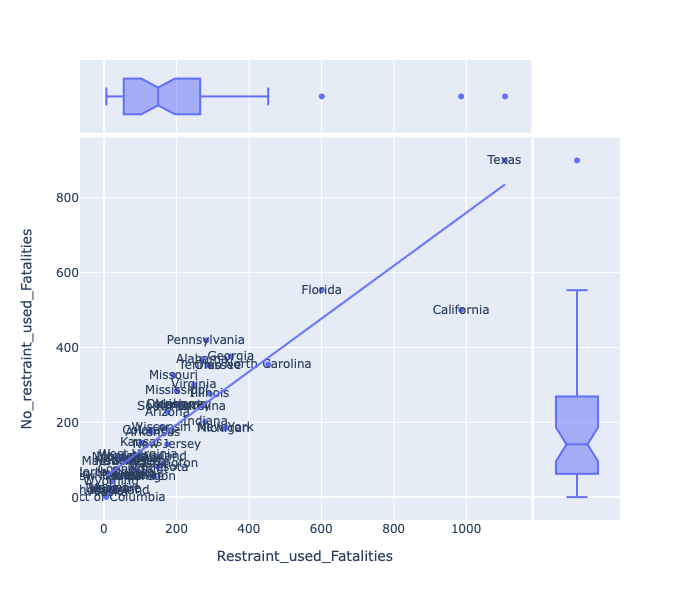
\includegraphics[width=.50\textwidth]{\MainFolder/Images/Fatal1.png}
    \caption{Scatterplot of fatal accident.}%\hrule
    \label{fig2a}
\end{figure}

\begin{figure}[H]
    \centering
    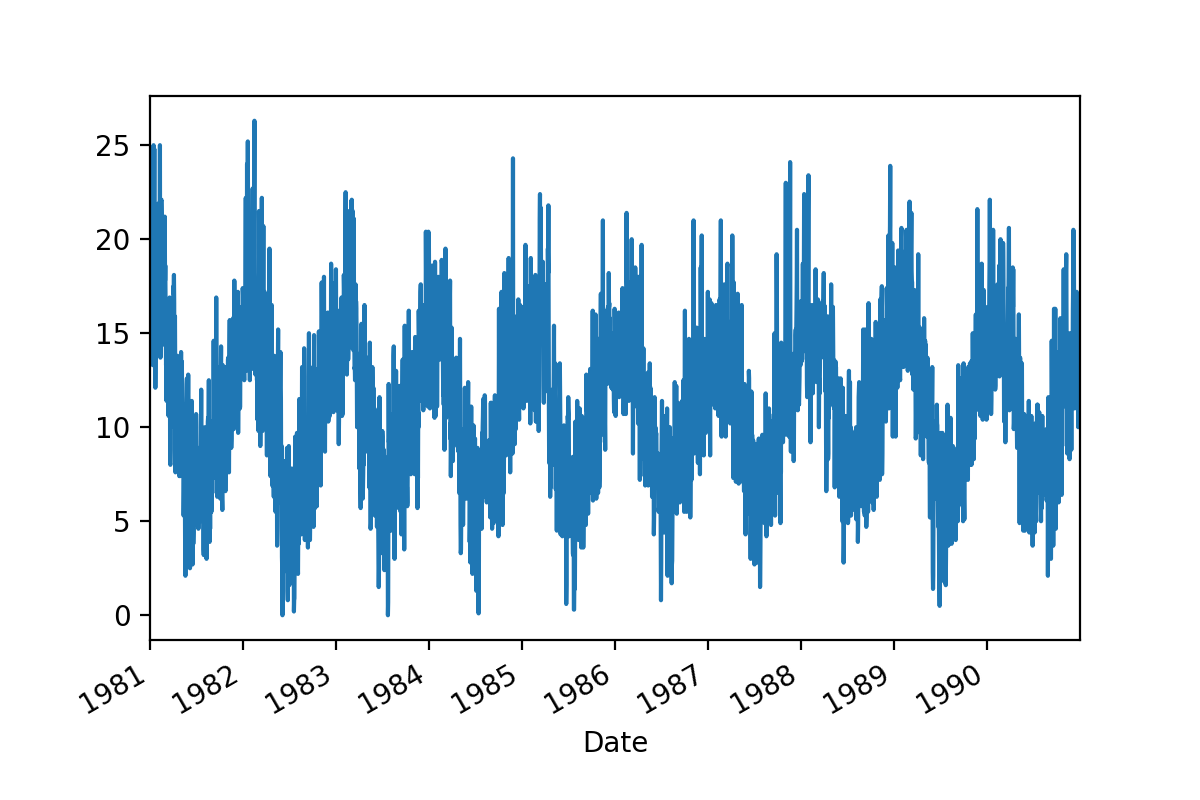
\includegraphics[width=.5\textwidth]{\MainFolder/Images/Temp1.png}
    %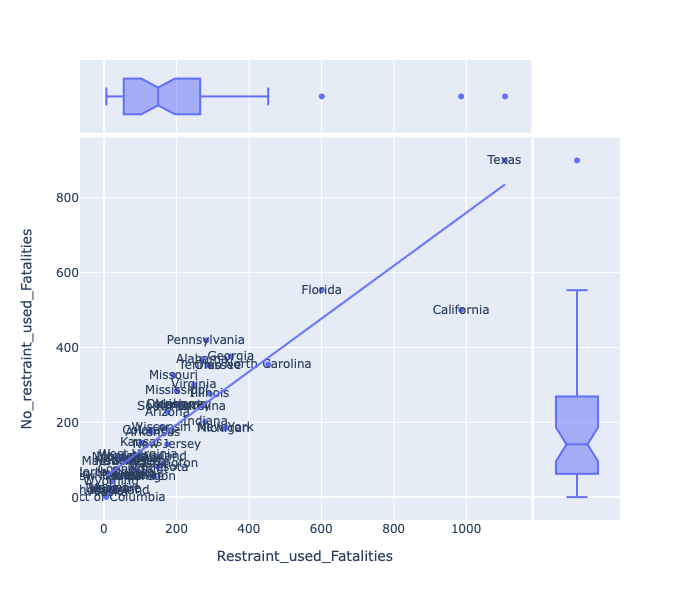
\includegraphics[width=.40\textwidth]{\MainFolder/Images/Fatal1.png}
    \caption{Daily minimum temperatures for the city of Melbourne, Australia (1981-1990).}%\hrule
    \label{fig2t}
\end{figure}




\noindent \textbf{e) Dataset 4: sale transactions:} this dataset contains information concerning the sales and products from \textbf{salespersonnel} from a certain company. The salespeople set their own selling prices and report the sales back to the company at the end of each month. A minor percentage of these records were audited and labeled as \textbf{"ok" or "fraud"}. It consists of $387010$ transactions, with 5 variable columns. After pre-treatment and removal of missing values, $15546$ observations are retained for further analysis with $1199$ fraudulent transactions i.e. $7 \%$. This is a supervised learning problem, the goal is the to train the model to correctly identify fraudulent and non-fraudulent transactions and predict the result for the remaining transactions. The data is available from the "DMwR" package in R.  

To evaluate the model's performance, these quantities are considered: \textbf{
Sensitivity, recall, or true positive rate; Specificity or true negative rate; Precision or positive predictive value; Negative predictive value; False positive rate; False negative rate; False discovery rate; Overall accuracy}, see Table \ref{fig_sale3}.

\noindent\textbf{Analysis of the results:} From Table \eqref{fig_sale3}, one can easily see that \textit{Isolation Forest (accuracy 91 $\%$)} and \textit{Local Outlier Factor (accuracy 87 $\%$)} outperform \textit{KNN (accuracy 9 $\%$)} and \textit{PCA (accuracy 13 $\%$)}.

Furthermore, the ROC (Receiver Operating Characteristic curve)\footnote{ROC curve, is a graphical plot of the sensitivity, or true positives, vs. (1 − specificity), or false positives, for a binary classifier system as its discrimination threshold is varied. The ROC can also be represented equivalently by plotting the fraction of true positives (TPR = true positive rate) vs. the fraction of false positives (FPR = false positive rate)}, and the \textbf{Area under the ROC curve or (AUC)}\footnote{ The AUC is a \textbf{visual} tool to measure the accuracy models and compare their performances. A \textbf{perfect} test correspond to an area of $1$ while a \textbf{bad} one correspond to an area of $.5$. A guide for classification is given by the academic point system: \textbf{
.90-1 = \textcolor{blue}{excellent (A)} ; .80-.90 = \textcolor{blue}{good (B)}; .70-.80 = \textcolor{blue}{fair (C)}; .60-.70 = \textcolor{blue}{poor (D)} et .50-.60 = \textcolor{blue}{fail (F)}}} (Figure \ref{fig_sal14})  provide tools to select possibly optimal models and to discard suboptimal ones independently from (and prior to specifying) the cost context or the class distribution \cite{ROC}. Indeed, from the graph \textbf{Isolation Forest} is a \textbf{good} model for this dataset with  AUC of $0.870$, followed by LOF with an AUC of $0.632$.
\begin{table}[H]
\centering
 \begin{tabular}{||l c c c c||} 
 \hline
 &  KNN & PCA & IsolForest & LOF\\ [0.5ex] 
 \hline\hline
Recall & 4 \% & 7 \%  & 95 \% & 93  \% \\ 
Specificity & 67 \% & 86 \%  & 43 \% & 18 \% \\
Precision & 58 \% & 86 \%  & 95 \% & 93 \% \\
NPV & 6 \% & 7 \%  & 44 \% & 18 \% \\
FP & 34 \% & 14 \%  & 57 \% & 82 \% \\
FN & 96 \% & 93 \%  & 5 \% & 7 \% \\
FD & 42 \% & 14 \%  & 5 \% & 7 \% \\
Accuracy & 9 \% & 13 \%  & \textcolor{blue}{91} \% & \textcolor{blue}{87} \% \\
[1ex] 
 \hline
 \end{tabular}
 \caption{Summary of results on sale transactions data set.}
 \label{fig_sale3}
\end{table}
%\end{figure*}
\begin{figure}[H]
    \centering
    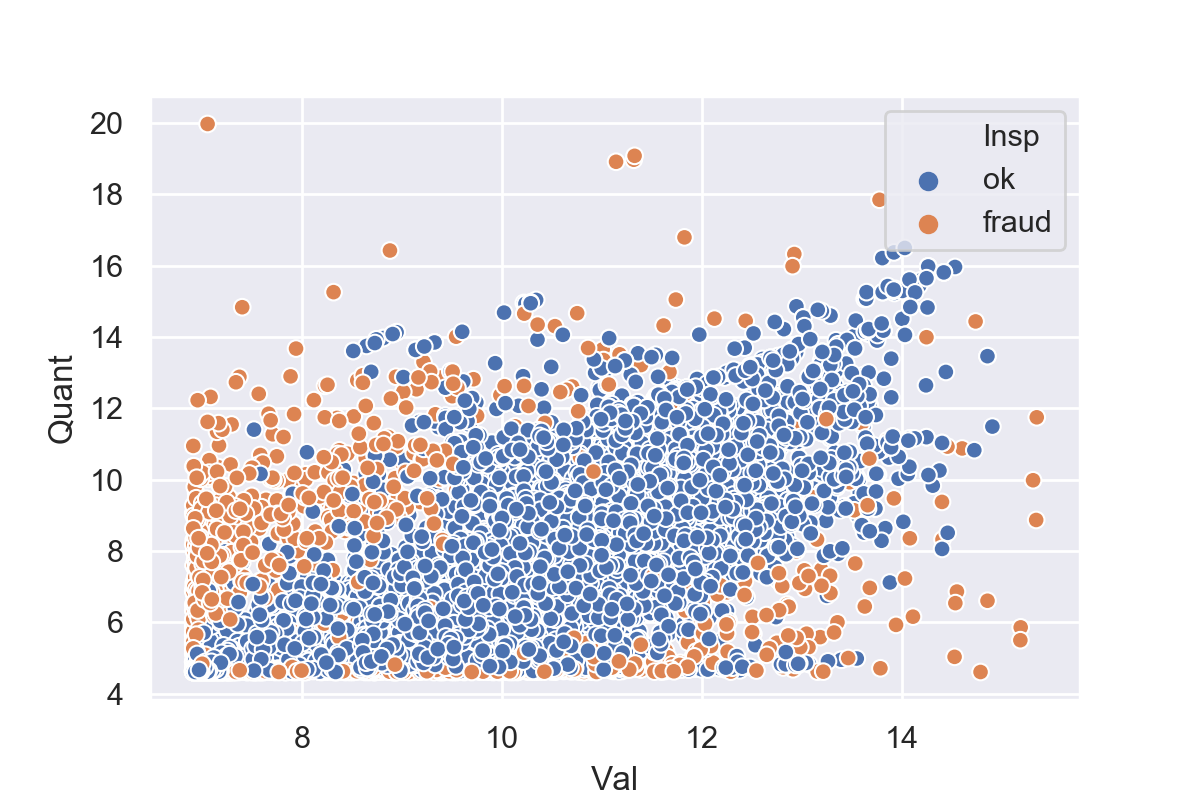
\includegraphics[width=.5\textwidth]{\MainFolder/Images/salescatter.png}
    \label{fig_sal11}
    %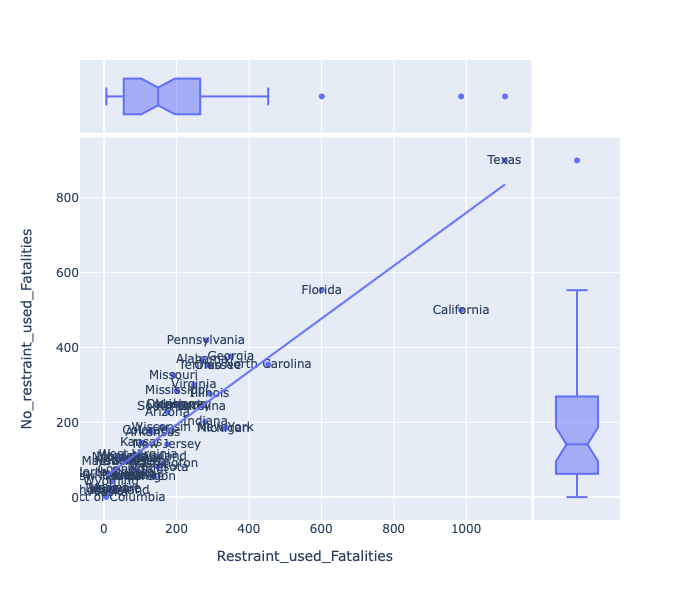
\includegraphics[width=.40\textwidth]{\MainFolder/Images/Fatal1.png}
    \caption{Scatterplot of sale transactions.}%\hrule
     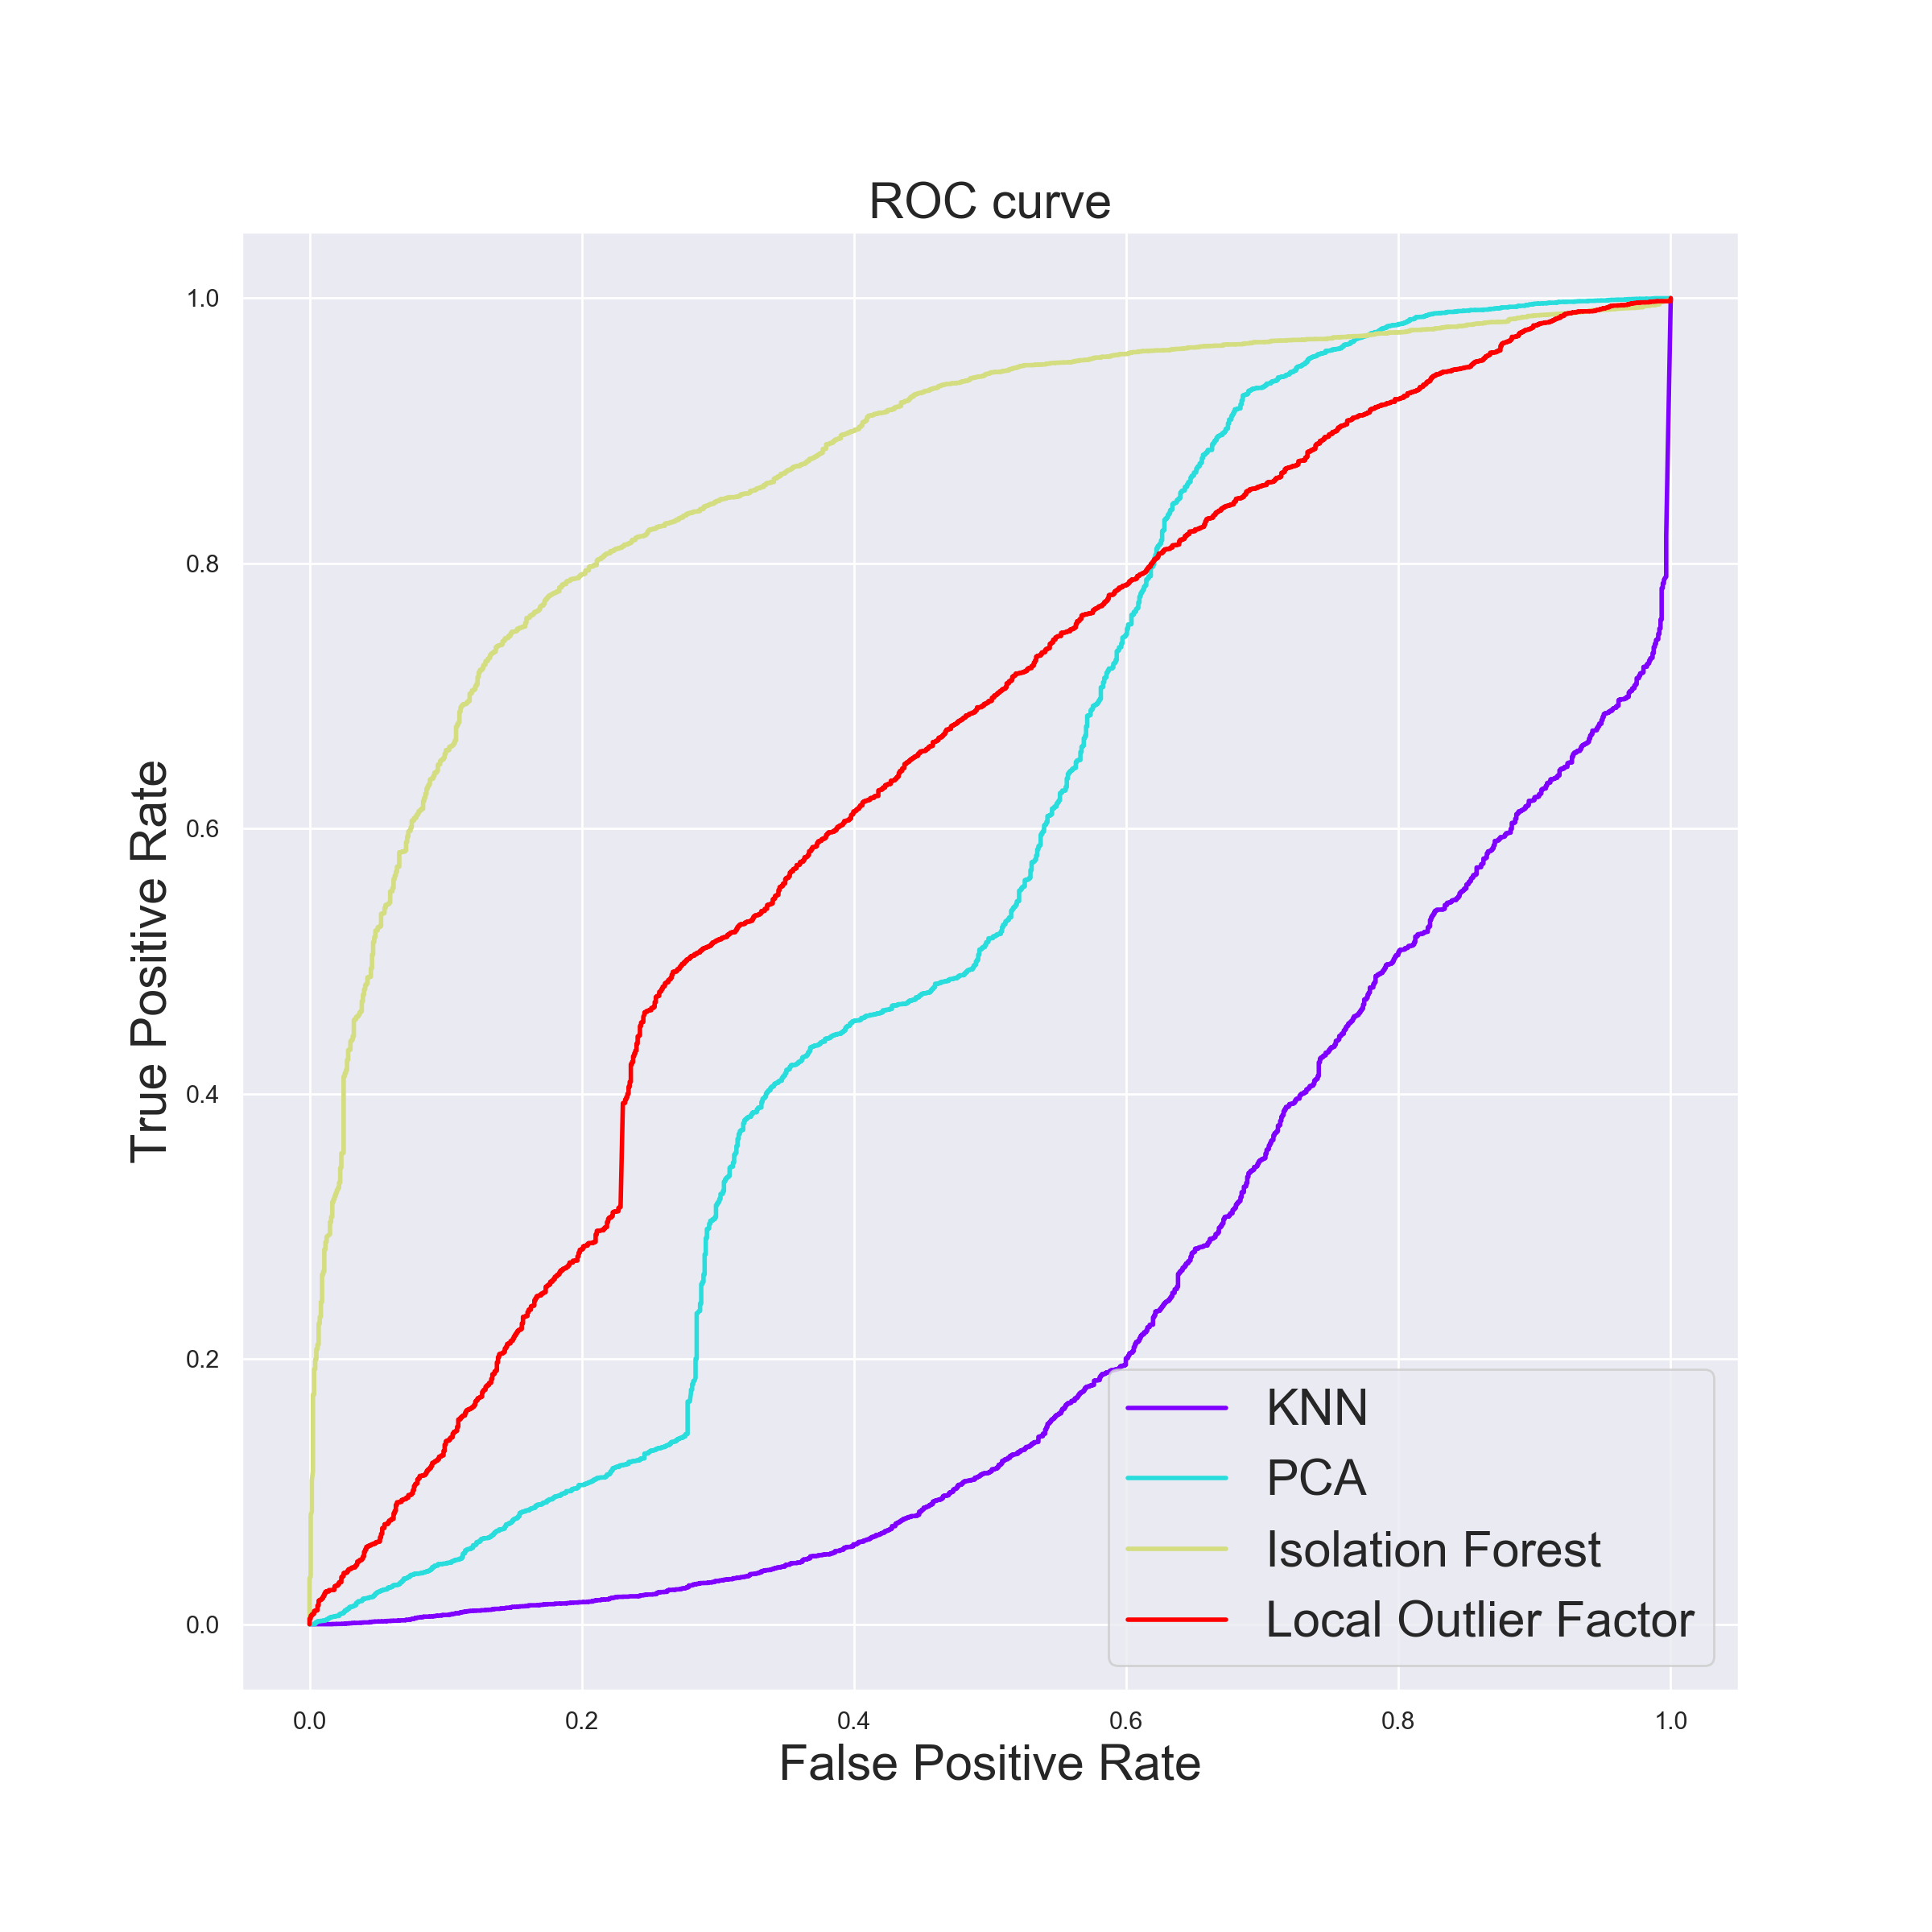
\includegraphics[width=.45\textwidth]{\MainFolder/Images/sales_roc.png}
     \caption{ROC Curve Plot for PCA, KNN, Isolation Forest, LOF.}%\hrul
     \label{fig_sal14}
\end{figure}
 \noindent However, PCA (AUC =$.56$) and KNN (AUC=$.23$) perform poorly. Figure \ref{fig_sal13} gives the confusion mwatrix of Isolation Forest. Out of $1119$ fraudulent transactions, it correctly identifies $521$ as such i.e. TP (sensitivity) of $43 \%$ and $678$ as normal  transactions i.e. FN rate of $ 57 \%$. Similarly, out of $15546$ normal transactions, it finds $13671$ as such i.e. TN (specificity) of $95 \%$  and $676$ as fraudulent i.e. FP  rate of $ 5\%$. 
\begin{figure}[H]
  
    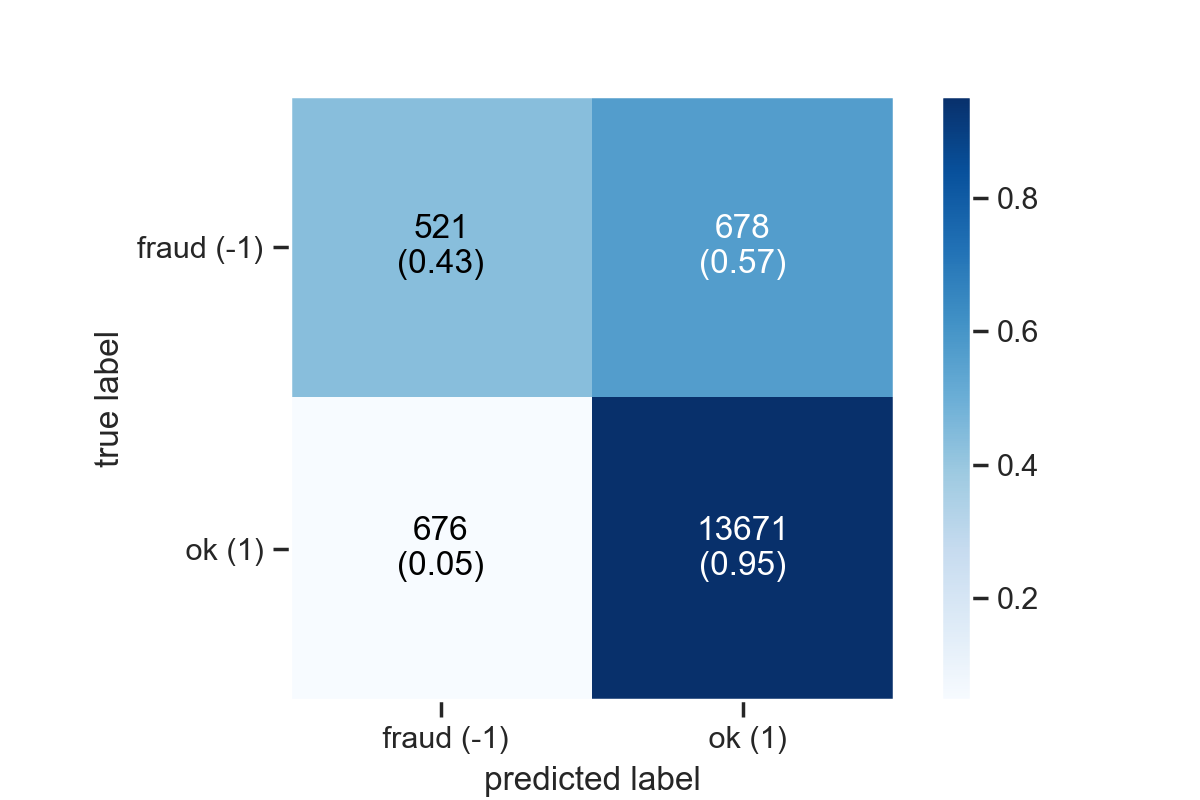
\includegraphics[width=.58\textwidth]{\MainFolder/Images/sales_confusionmat.png}
  \caption{Confusion matrix for Isolation Forest.}
    \label{fig_sal13}
\end{figure}

%\begin{figure}[H]
    %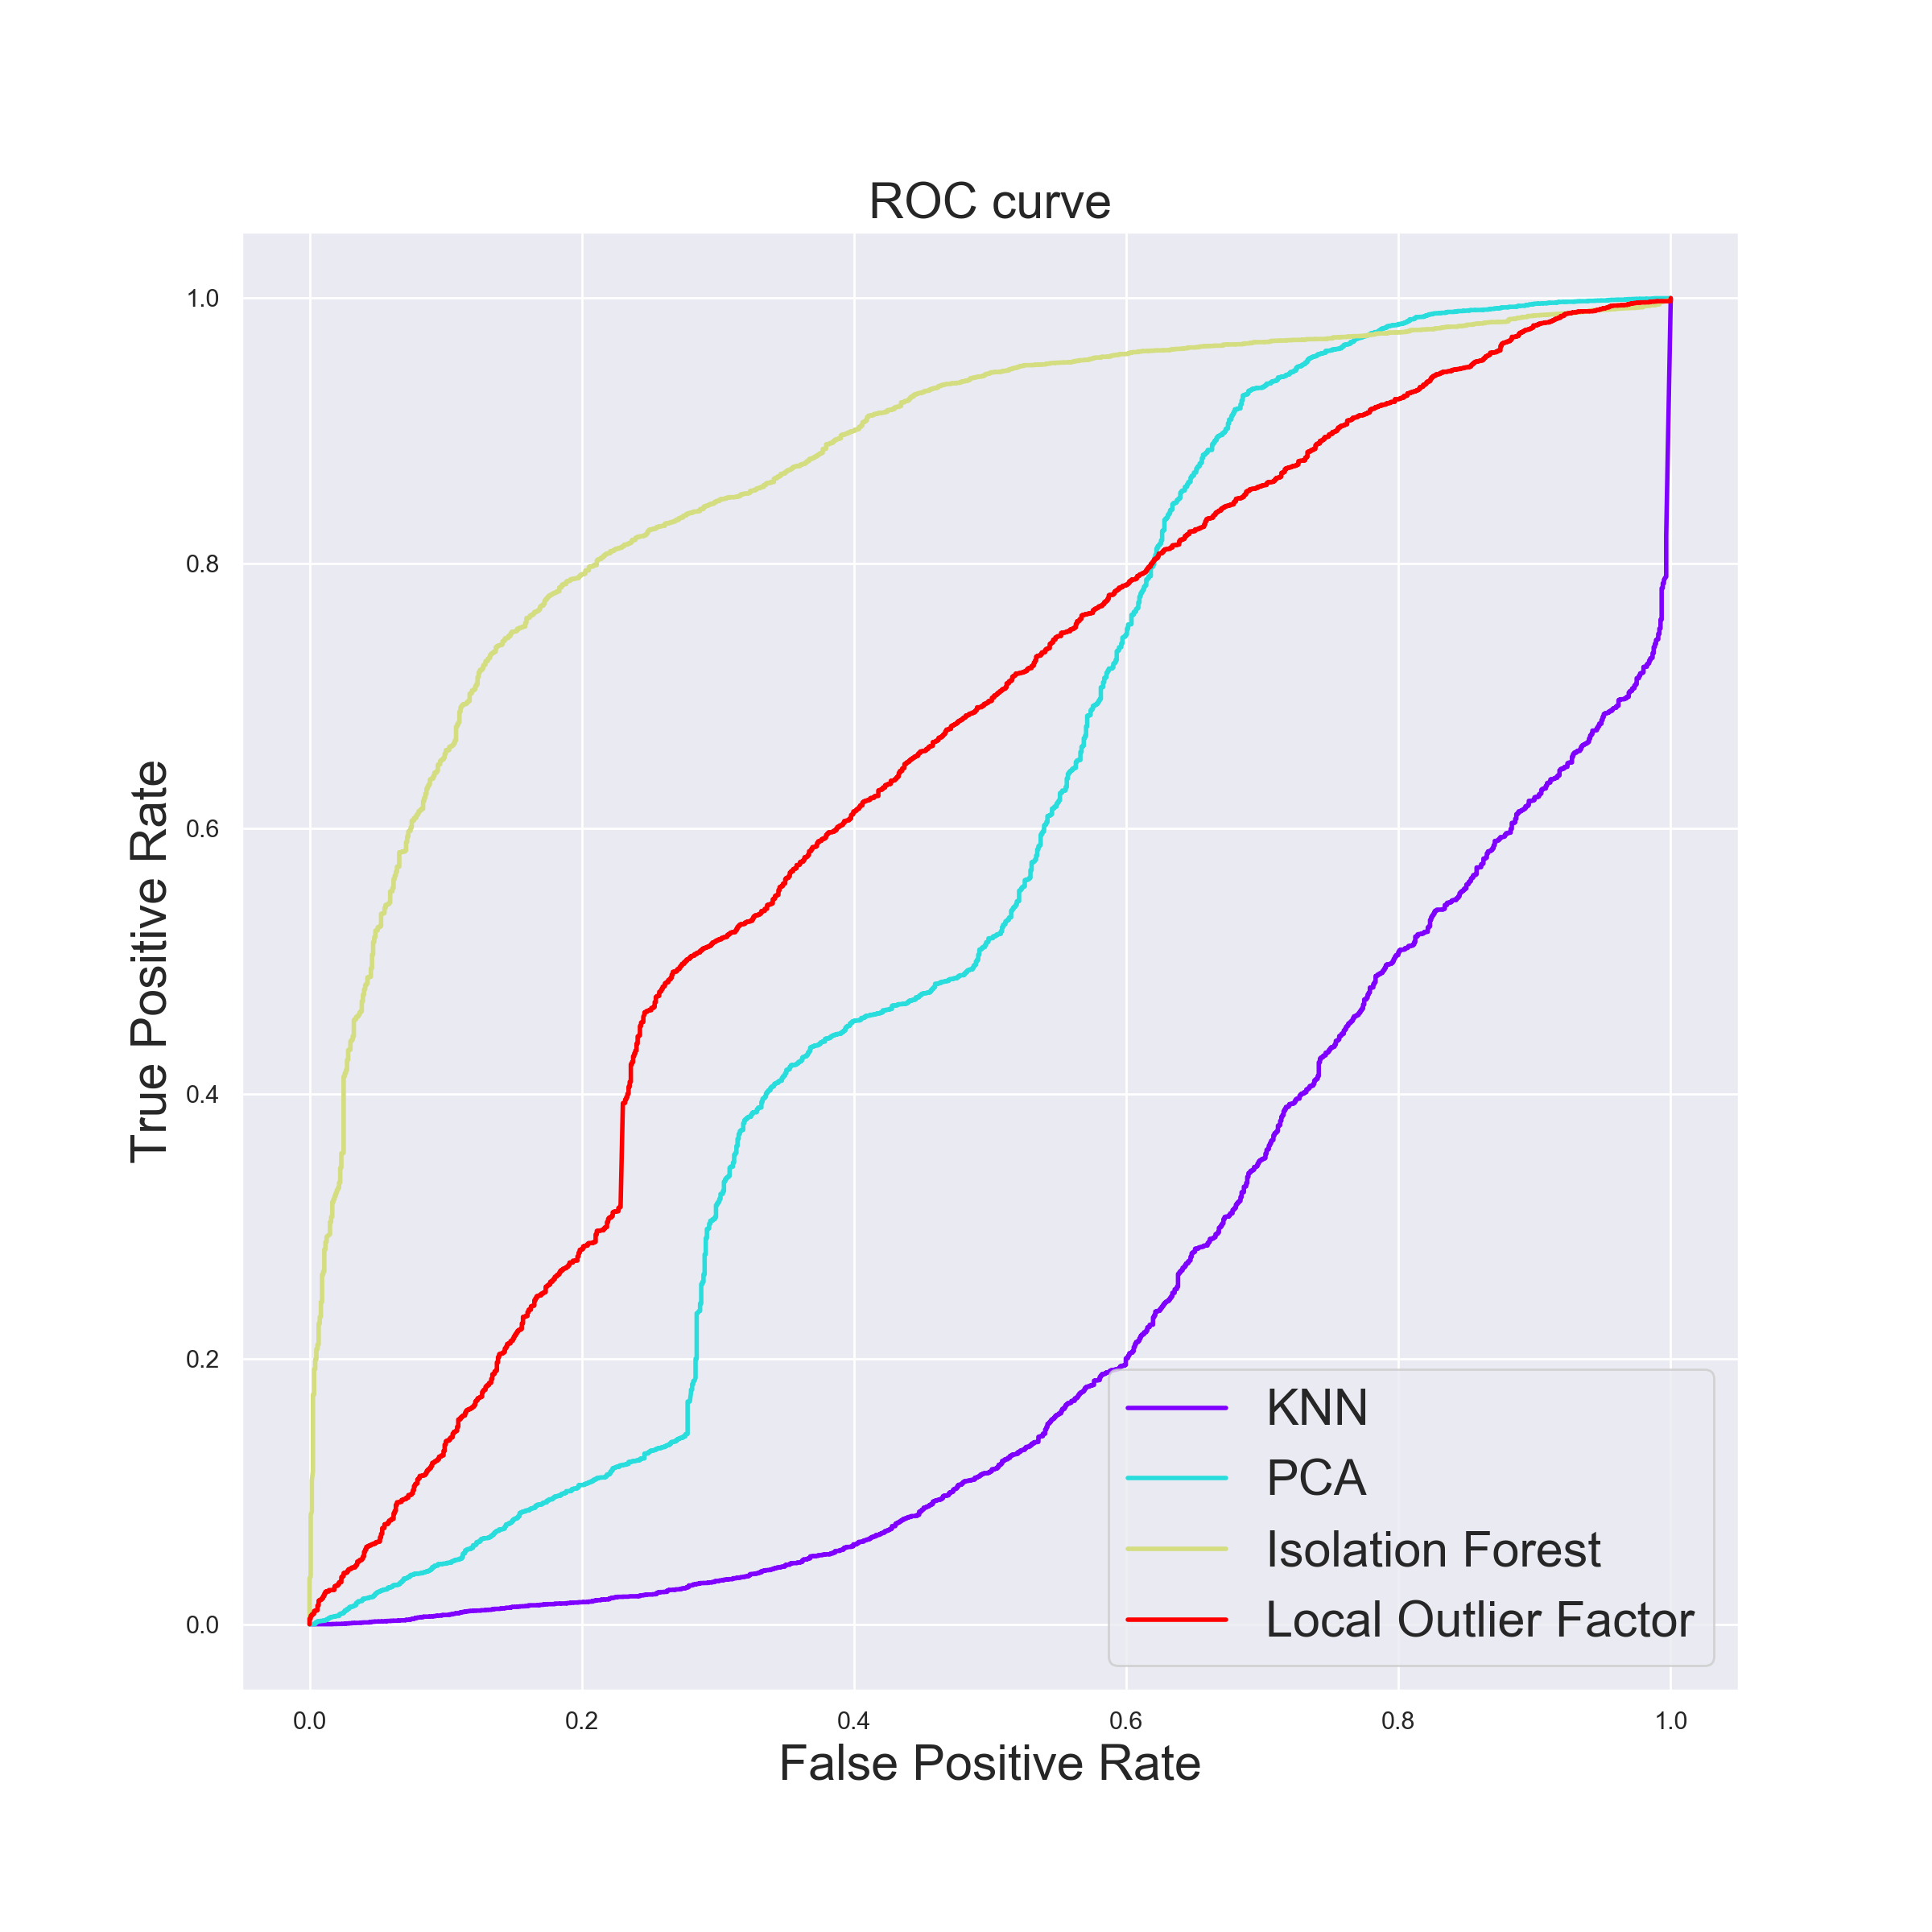
\includegraphics[width=.40\textwidth]{\MainFolder/Images/sales_roc.png}
 %   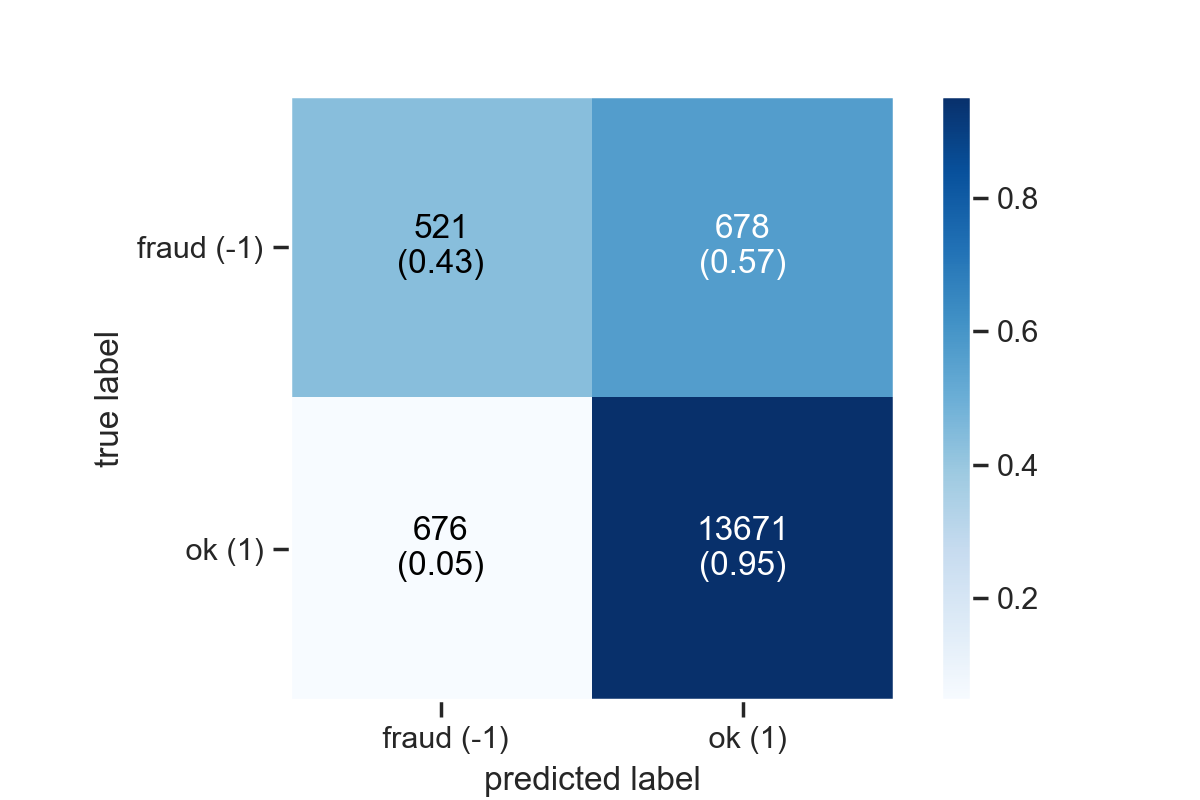
\includegraphics[width=.6\textwidth]{\MainFolder/Images/sales_confusionmat.png}
  %  \caption{Confusion matrix fro Isolation Forest (right).}%\hrul
   % \label{fig_sal13}
%\end{figure}
\begin{figure}[H]
    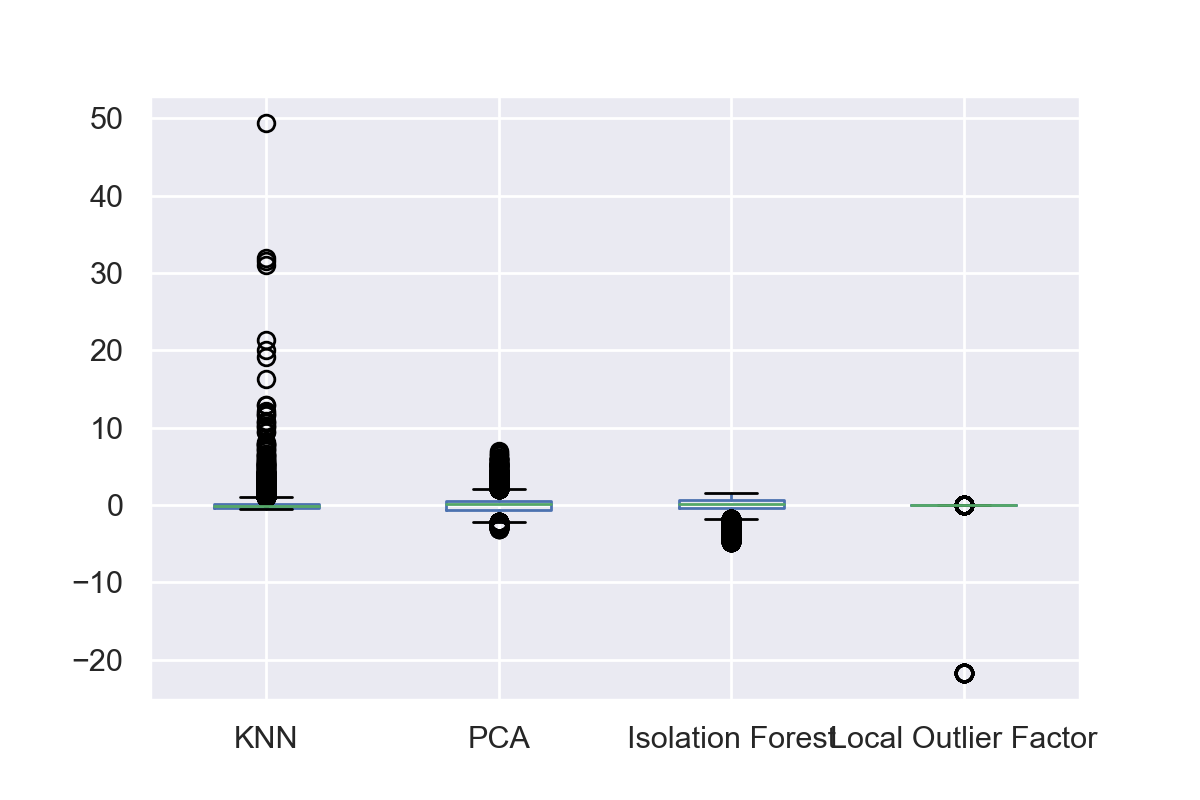
\includegraphics[width=.45\textwidth]{\MainFolder/Images/sales_boxplot.png}
    \label{fig_sal12}
    \caption{Boxplot of the performences of PCA, KNN, Isolation Forest, LOF.}%\hrule
\end{figure}


\begin{figure*}[ht!]
    \centering
    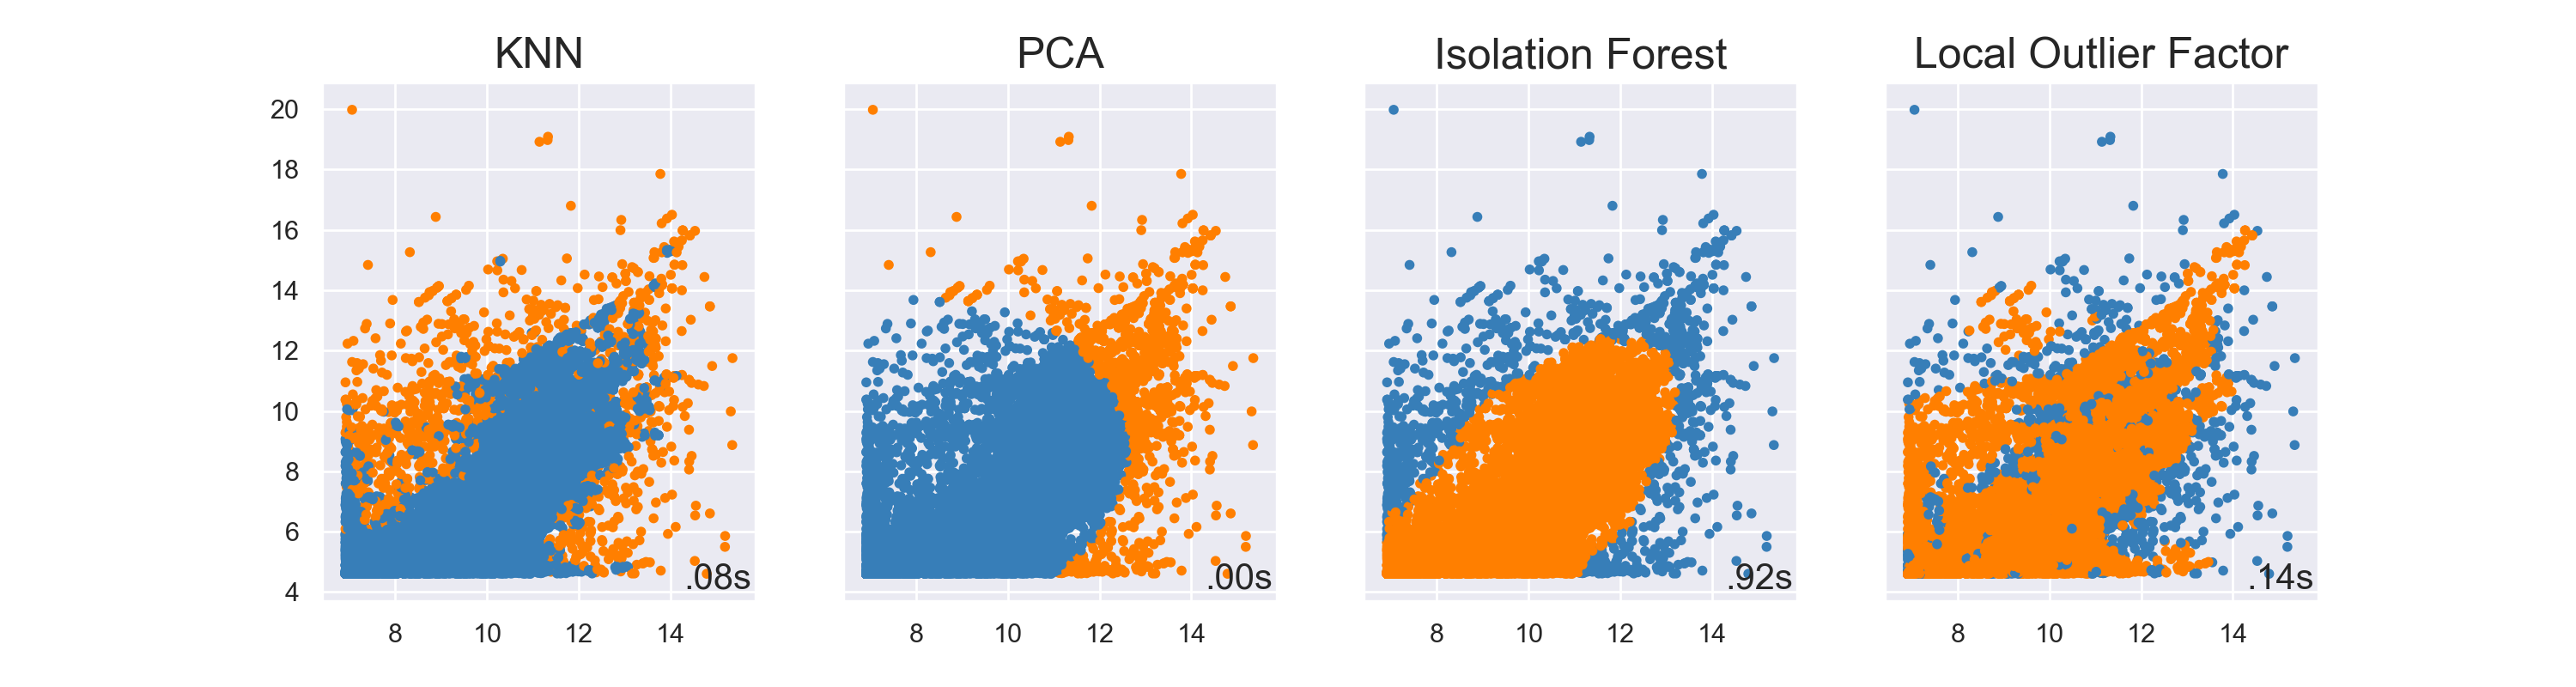
\includegraphics[width=1.06\textwidth]{\MainFolder/Images/sale_algo.png}
    \caption{Fraudulent transactions detected as outliers by PCA, KNN, Isolation Forest and LOF.}%\hrule
    \label{fig_sal2}
    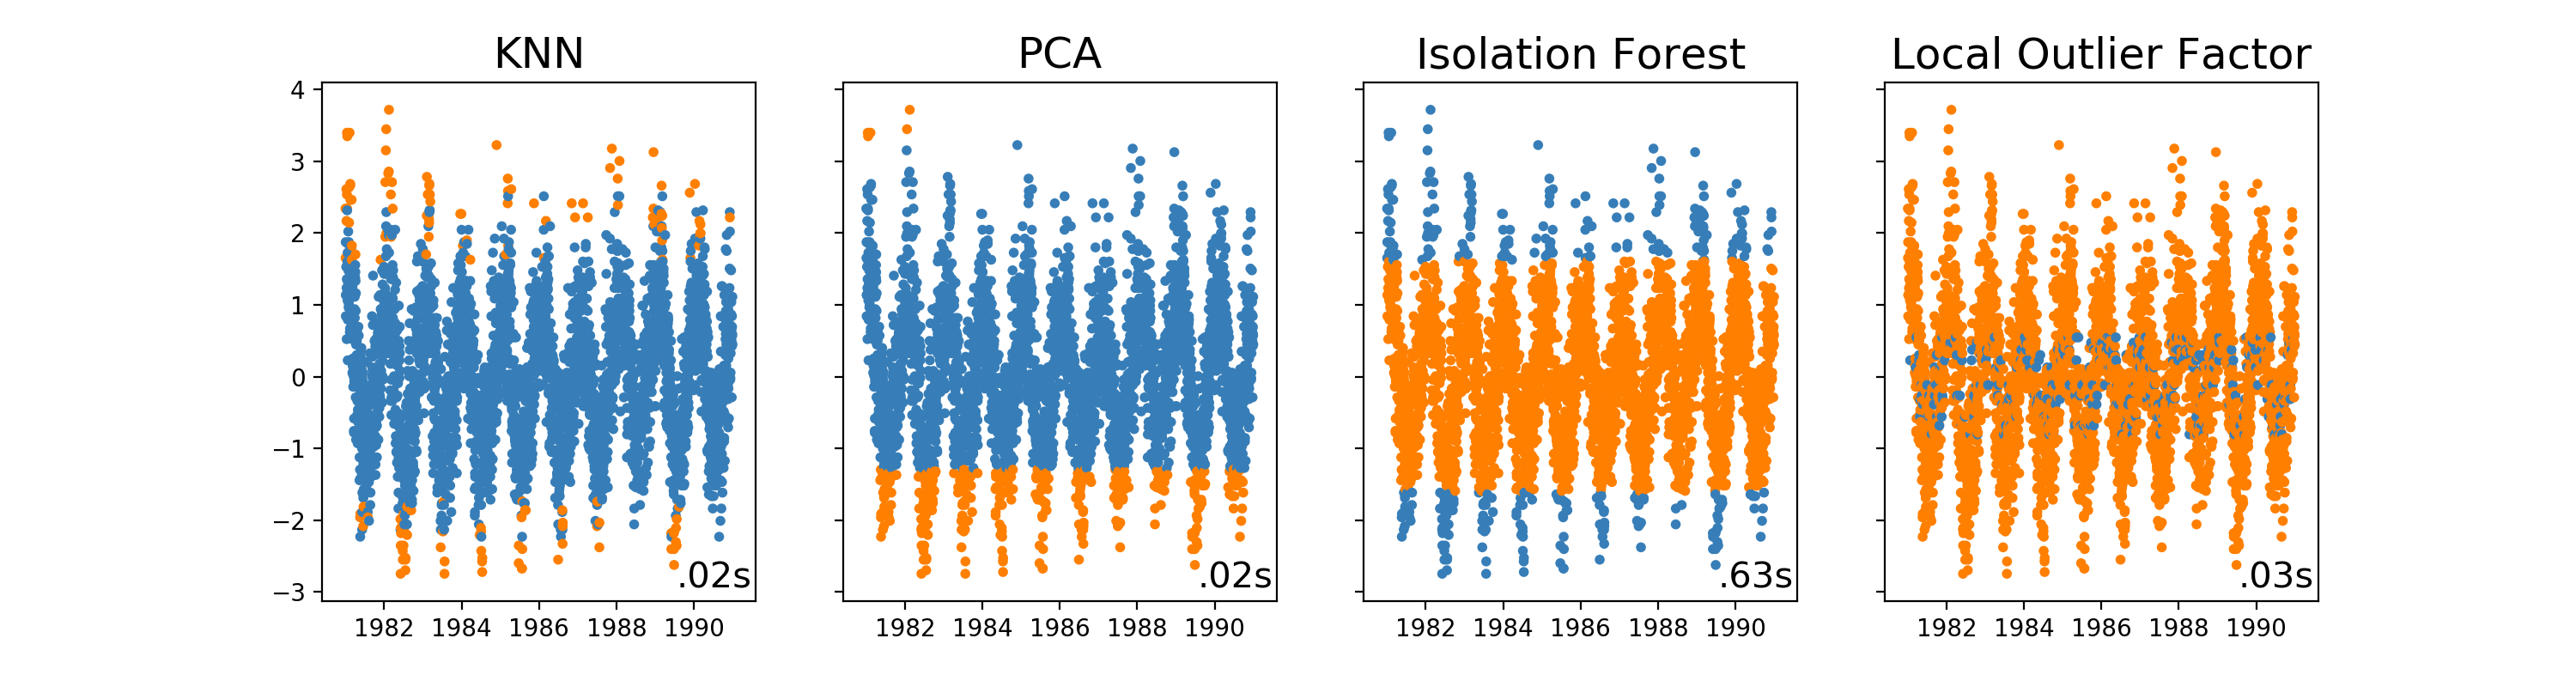
\includegraphics[width=1.06\textwidth]{\MainFolder/Images/Temp2.png}
    \caption{Temperatures detected as outliers by PCA, KNN, Isolation Forest and LOF.}%\hrule
    \label{fig2t1}
\end{figure*}
\begin{figure*}[ht!]
 \centering
     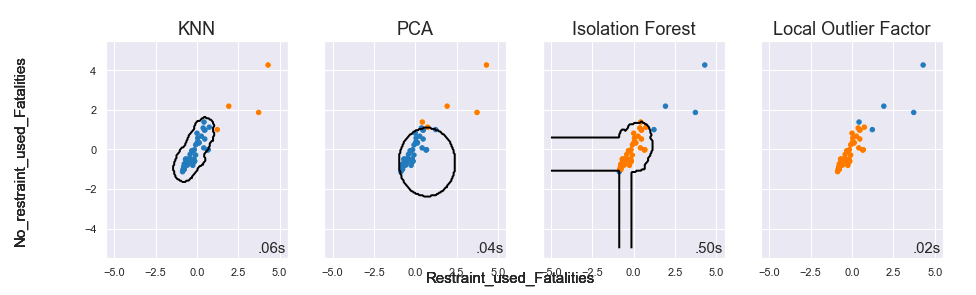
\includegraphics[width=1\textwidth]{\MainFolder/Images/Fatal11.png}
    \caption{Illustration des performences des méthodes: KNN, PCA, Isolation forest and LOF}%\hrule
    \label{fig3}
\end{figure*}

\begin{figure*}[ht]
    \centering
    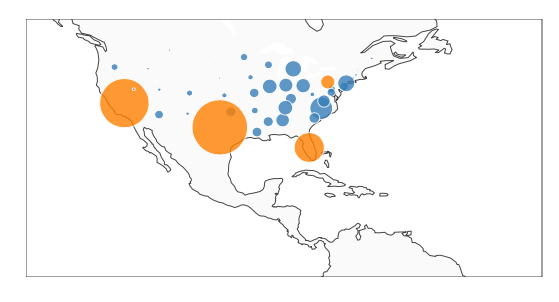
\includegraphics[width=.45\textwidth]{\MainFolder/Images/FatPCA.png}
    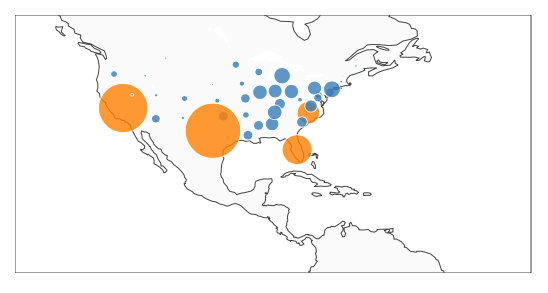
\includegraphics[width=.450\textwidth]{\MainFolder/Images/FatKNN.png}\\
    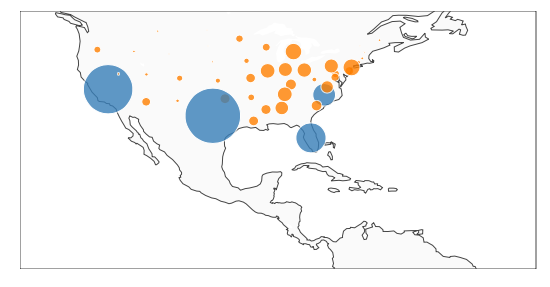
\includegraphics[width=.45\textwidth]{\MainFolder/Images/FatIsofore.png}
    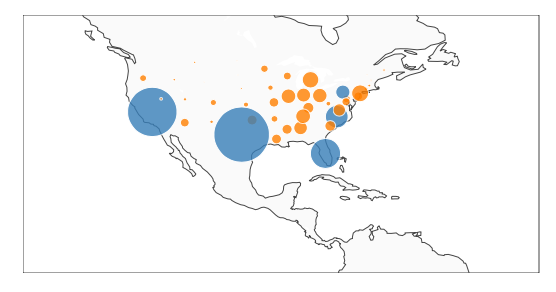
\includegraphics[width=.450\textwidth]{\MainFolder/Images/FatLOF.png}
    \caption{Villes qui ont plus d'accidents mortels détectées comme aberrantes par PCA (en haut à gauche), KNN (en haut à droite), Isolation Forest (en bas à gauche) et LOF (en bas à droite)}%\hrule
    \label{fig2b}
\end{figure*}


\afterpage{\FloatBarrier}